\title{Lausnir á dæmum tengd viku fjögur}
\author{Bergur Snorrason}
\date{\today}

\begin{document}

\frame{\titlepage}

\env{frame}
{
	\env{itemize}
	{
		\item<1-> Ég mun leysa eftirfarandi dæmi:
		\env{itemize}
		{
			\item<2-> \emph{Kaffi},
			\item<3-> \emph{Bad Packing}.
		}
	}
}

\env{frame}
{
	\frametitle{Kaffi}
	\env{itemize}
	{
		\item<1-> Við erum með litla kassa sem við viljum stafla við vegg sem er með takmarkaða breidd.
		\item<2-> Hver kassi hefur lit og kassar af mismunandi litum mega ekki staflast ofan á hvorn annan.
		\item<3-> Við viljum lágmarka svæðið á veggnum sem sést fyrir aftan stöfluðu kassana.
		\item<4->[] 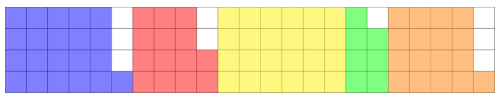
\includegraphics[scale = 0.5]{fig/kaffi.png}
	}
}

\env{frame}
{
	\frametitle{Kaffi}
	\env{itemize}
	{
		\item<1-> Látum gefnu breiddina vera $w$.
		\item<2-> Flatarmálið sem við viljum lágmarka er heildarflatarmálið mínus flatarmál kassana.
		\item<3-> En kassarnir hafa fast flatarmál, svo okkur nægir að lágmarka heildarflatarmálið.
		\item<4-> Þar sem breddin er föst nægir okkur að lágmarka hæðina.
		\item<5-> Svo okkur nægir að finna minnstu hæðina $h$ þannig að það megi stafla kössunum í $w$ stafla og hver stafli er hefur mest $h$ kassa.
		\item<6-> Tökum þó eftir að ef þetta er hægt fyrir $h$ þá er þetta líka hægt fyrir $h' > h$.
		\item<7-> Svo við getum notað helmingunarleit til að finn minnstu hæðina.
	}
}

\env{frame}
{
	\frametitle{Kaffi}
	\env{itemize}
	{
		\item<1-> Hvernig athugum við hvort gefin hæð $h$ sé nógu há.
		\item<2-> Gerum ráð fyrir kassarnir hafi $n$ mismunandi liti og $a_i$ kassar séu af $i$-ta litnum.
		\item<3-> Við þurfum þá $\lceil a_i/h \rceil$ stafla fyrir kassa af lit $i$.
		\item<4-> Svo $h$ er nógu stórt ef
		\[
			\sum_{i = 1}^n \lceil a_i/h \rceil \leq w.
		\]
	}
}

\env{frame}
{
	\frametitle{Kaffi}
	\code{code/kaffi.c}
}

\env{frame}
{
	\frametitle{Kaffi}
	\env{itemize}
	{
		\item<1-> Við erum $\mathcal{O}($\onslide<2->{$\,n\,$}$)$ tíma að ganga úr skugga um það hvort tiltekin hæð sé nógu há.
		\item<3-> Með helmingunarleitinn verður tímaflækjan $\mathcal{O}($\onslide<4->{$n \log m$}$)$,
					þar sem $m$ er mesti mögulegi fjöldi stóla af hverjum lit.
	}
}

\env{frame}
{
	\frametitle{Bad Packing}
	\env{itemize}
	{
		\item<1-> Við erum með $n \leq 10^3$ hluti, hlutirnir hafa þyngdir $w_1, \dots, d_n$ og bakpoka sem rúmar $c \leq 10^5$ samtals þyngd.
		\item<2-> Ef við veljum hluti af handahófi þangað til bakpokinn okkar rúmar ekki fleiri hluti, hver er þá minnsta þyngdin sem við getum endað með.
		\item<3-> Til dæmis, ef $n = 3$, $c = 6$ og við hofum þyngdir $3$, $3$ og $4$ þá gætum við endað með þyngdir $3 + 3 = 6$ og $5$.
	}
}

\env{frame}
{
	\frametitle{Bad Packing}
	\env{itemize}
	{
		\item<1-> Þetta dæmi minnir mjög á hlutmengjasummu dæmið.
		\item<2-> Rifjum upp að við létum $f(i, j)$ vera $1$ ef einhver hlutruna $w_1, \dots, w_i$ hafi summu $j$ og $f$ hefur rakningarformúlu
		\[
			f(i, j) =
			\left \{
			\env{array}
			{
				{l l}
				1, & \text{ef $i = 0$ og $j = 0$},\\
				0, & \text{ef $i = 0$ og $j \neq 0$, eða $j < 0$},\\
				f(i - 1, j) \text{ eða }\\
					\quad f(i - 1, j - a_i)), & \text{ef $i \neq 0$}.
			}
			\right .
		\]
	}
}

\env{frame}
{
	\frametitle{Bad Packing}
	\env{itemize}
	{
		\item<1-> Reynum að svara spurningunni: ,,Er mögulegt að enda með þyngd $k$?''.
		\item<2-> Tökum eftir að við þurfum alltaf að taka alla hluti sem hafa þyngd minni eða jafna $k$.
		\item<3-> Ef við tökum ekki þá hluti þá gætum við bætt þeim í bakpokann okkar.
		\item<4-> Látum $s$ vera summu allra hlutanna sem hafa þyngd minni eða jafna $k$.
		\item<5-> Við þurfum þá að svara spurningunni: ,,Getum við valið hluti, alla þyngri en $k$, sem hafa summu $k - s$?''.
		\item<6-> Þetta er hlutmengjasummudæmi, en við þurfum þó að passa okkur.
		\item<7-> Ef við notum beint kóðann úr síðasta fyrirlestri og gerum þetta fyrir hverja þyngd fæst tímaflækjan $\mathcal{O}(nc^2)$,
					sem er alltof hægt.
	}
}

\env{frame}
{
	\frametitle{Bad Packing}
	\env{itemize}
	{
		\item<1-> Þessi slæma tímaflækja fæst þó því við leysum hlutmengjasummudæmið $c$ sinnum.
		\item<2-> Rifjum upp að
		\[
			f(i, j) =
			\left \{
			\env{array}
			{
				{l l}
				1, & \text{ef $i = 0$ og $j = 0$},\\
				0, & \text{ef $i = 0$ og $j \neq 0$, eða $j < 0$},\\
				f(i - 1, j) \text{ eða }\\
					\quad f(i - 1, j - a_i)), & \text{ef $i \neq 0$}.
			}
			\right .
		\]
		\item<3-> Tökum eftir að eftir að hafa leyst hlutmengjasummu dæmið einu sinni höfum við í raun leyst það fyrir öll söfn vigta
					af gerðinni $w_1, \dots, w_k$.
		\item<4-> Ef við röðum vigtunum okkar í minnkandi röð þurfum við bara að leysa hlutmengjasummudæmið einu sinni.
	}
}

\env{frame}
{
	\frametitle{Bad Packing}
	\selectcode{code/badpacking.c}{11}{37}
}

\env{frame}
{
	\frametitle{Bad Packing}
	\env{itemize}
	{
		\item<1-> Við röðum $n$ tölum sem tekur $\mathcal{O}($\onslide<2->{$n \log n$}$)$.
		\item<3-> Við þurfum líka að leysa hlutmengjasummudæmið, sem tekur $\mathcal{O}($\onslide<4->{$c \cdot n$}$)$.
		\item<5-> Við höfum að lokum tvöfalda \texttt{for}-lykkju,
					sú ytri af lengd $\mathcal{O}(\,c\,)$ og sú innri af lengd $\mathcal{O}(\,n\,)$,
					og samtals er þetta $\mathcal{O}($\onslide<6->{$c \cdot n$}$)$.
		\item<7-> Samtals er þetta forrit því $\mathcal{O}($\onslide<8->{$c \cdot n$}$)$.
	}
}

\env{frame}
{
}

\end{document}
